\documentclass[conference]{IEEEtran}

\usepackage[utf8]{inputenc}
\usepackage[T1]{fontenc}
\usepackage{graphicx}
\usepackage{amsmath}
\usepackage{hyperref}
\usepackage{listings}
\usepackage{xcolor}
\usepackage{booktabs}
\usepackage{caption}
\usepackage{tikz}
\usetikzlibrary{positioning}

% ---------- code listing style ----------
% One shared style for GLSL and JavaScript snippets. GLSL isn't a built-in
% listings language, so its keywords are declared manually below.
\lstdefinelanguage{GLSL}{
  keywords={vec2,vec3,vec4,mat4,float,int,void,uniform,varying,attribute,
            precision,highp,mediump,lowp,if,else,for,return,const,bool,true,false},
  keywordstyle=\color{blue}\bfseries,
  comment=[l]{//},
  commentstyle=\color{gray}\itshape,
  morestring=[b]",
  stringstyle=\color{orange},
  sensitive=true
}

\lstset{
  basicstyle=\ttfamily\footnotesize,
  numbers=left,
  numberstyle=\tiny\color{gray},
  frame=single,
  breaklines=true,
  showstringspaces=false,
  captionpos=b,
  backgroundcolor=\color{black!3}
}

\begin{document}

\title{Let Me Ask Charlie: A Procedural Real-Time Lighting and Shadow Pipeline for Browser-Based Interactive Horror}

\author{
  \IEEEauthorblockN{Ashmit Deb Roy}
  \IEEEauthorblockA{DH2323 Computer Graphics and Interaction \\ KTH Royal Institute of Technology}
}

\maketitle

\begin{abstract}
\textit{Let Me Ask Charlie} is a browser-based interactive vignette built around a custom real-time lighting and shadow pipeline rather than an off-the-shelf game engine renderer. The environment's surface normals are derived procedurally in a GLSL fragment shader from a greyscale height map using a Sobel gradient; no pre-authored normal map exists anywhere in the project. Lambertian ($N\cdot L$) diffuse shading, a signed-distance-field (SDF) soft-shadow raymarcher extended to a shared scene distance field covering both the moving antagonist and static furniture, and a four-effect post-processing pass (bloom, Reinhard tone mapping, vignette, hash-based film grain) complete the pipeline. All characters are drawn procedurally with no image or sprite-sheet assets. A short evaluation compares the full lit pipeline against an unlit control build using the Self-Assessment Manikin, isolating the rendering technique itself as the variable under test rather than evaluating the experience as a whole. Across $n=8$ within-subjects sessions, the lit condition scored directionally higher than flat on all three SAM dimensions (valence, arousal, dominance), though only as a suggestive, exploratory signal at this sample size rather than a statistically powered result; open-ended responses suggest the technique changes what participants attend to, not simply how afraid they feel.
\end{abstract}

\begin{IEEEkeywords}
real-time rendering, signed distance fields, soft shadows, procedural normal mapping, shader programming, interactive horror, self-assessment manikin
\end{IEEEkeywords}

\section{Introduction}
\textit{Let Me Ask Charlie} explores an interactive experience in which a user is pursued through a single room by an antagonist rendered entirely as mathematics: no sprite, no pre-rendered animation, only a signed distance field whose shadow grows as it approaches. The project is implemented as a custom browser application (p5.js + GLSL) rather than a full-featured game engine project, which foregrounds deliberate technical and design choices in rendering, interaction, and system architecture over asset production.

\begin{figure}[t]
  \centering
  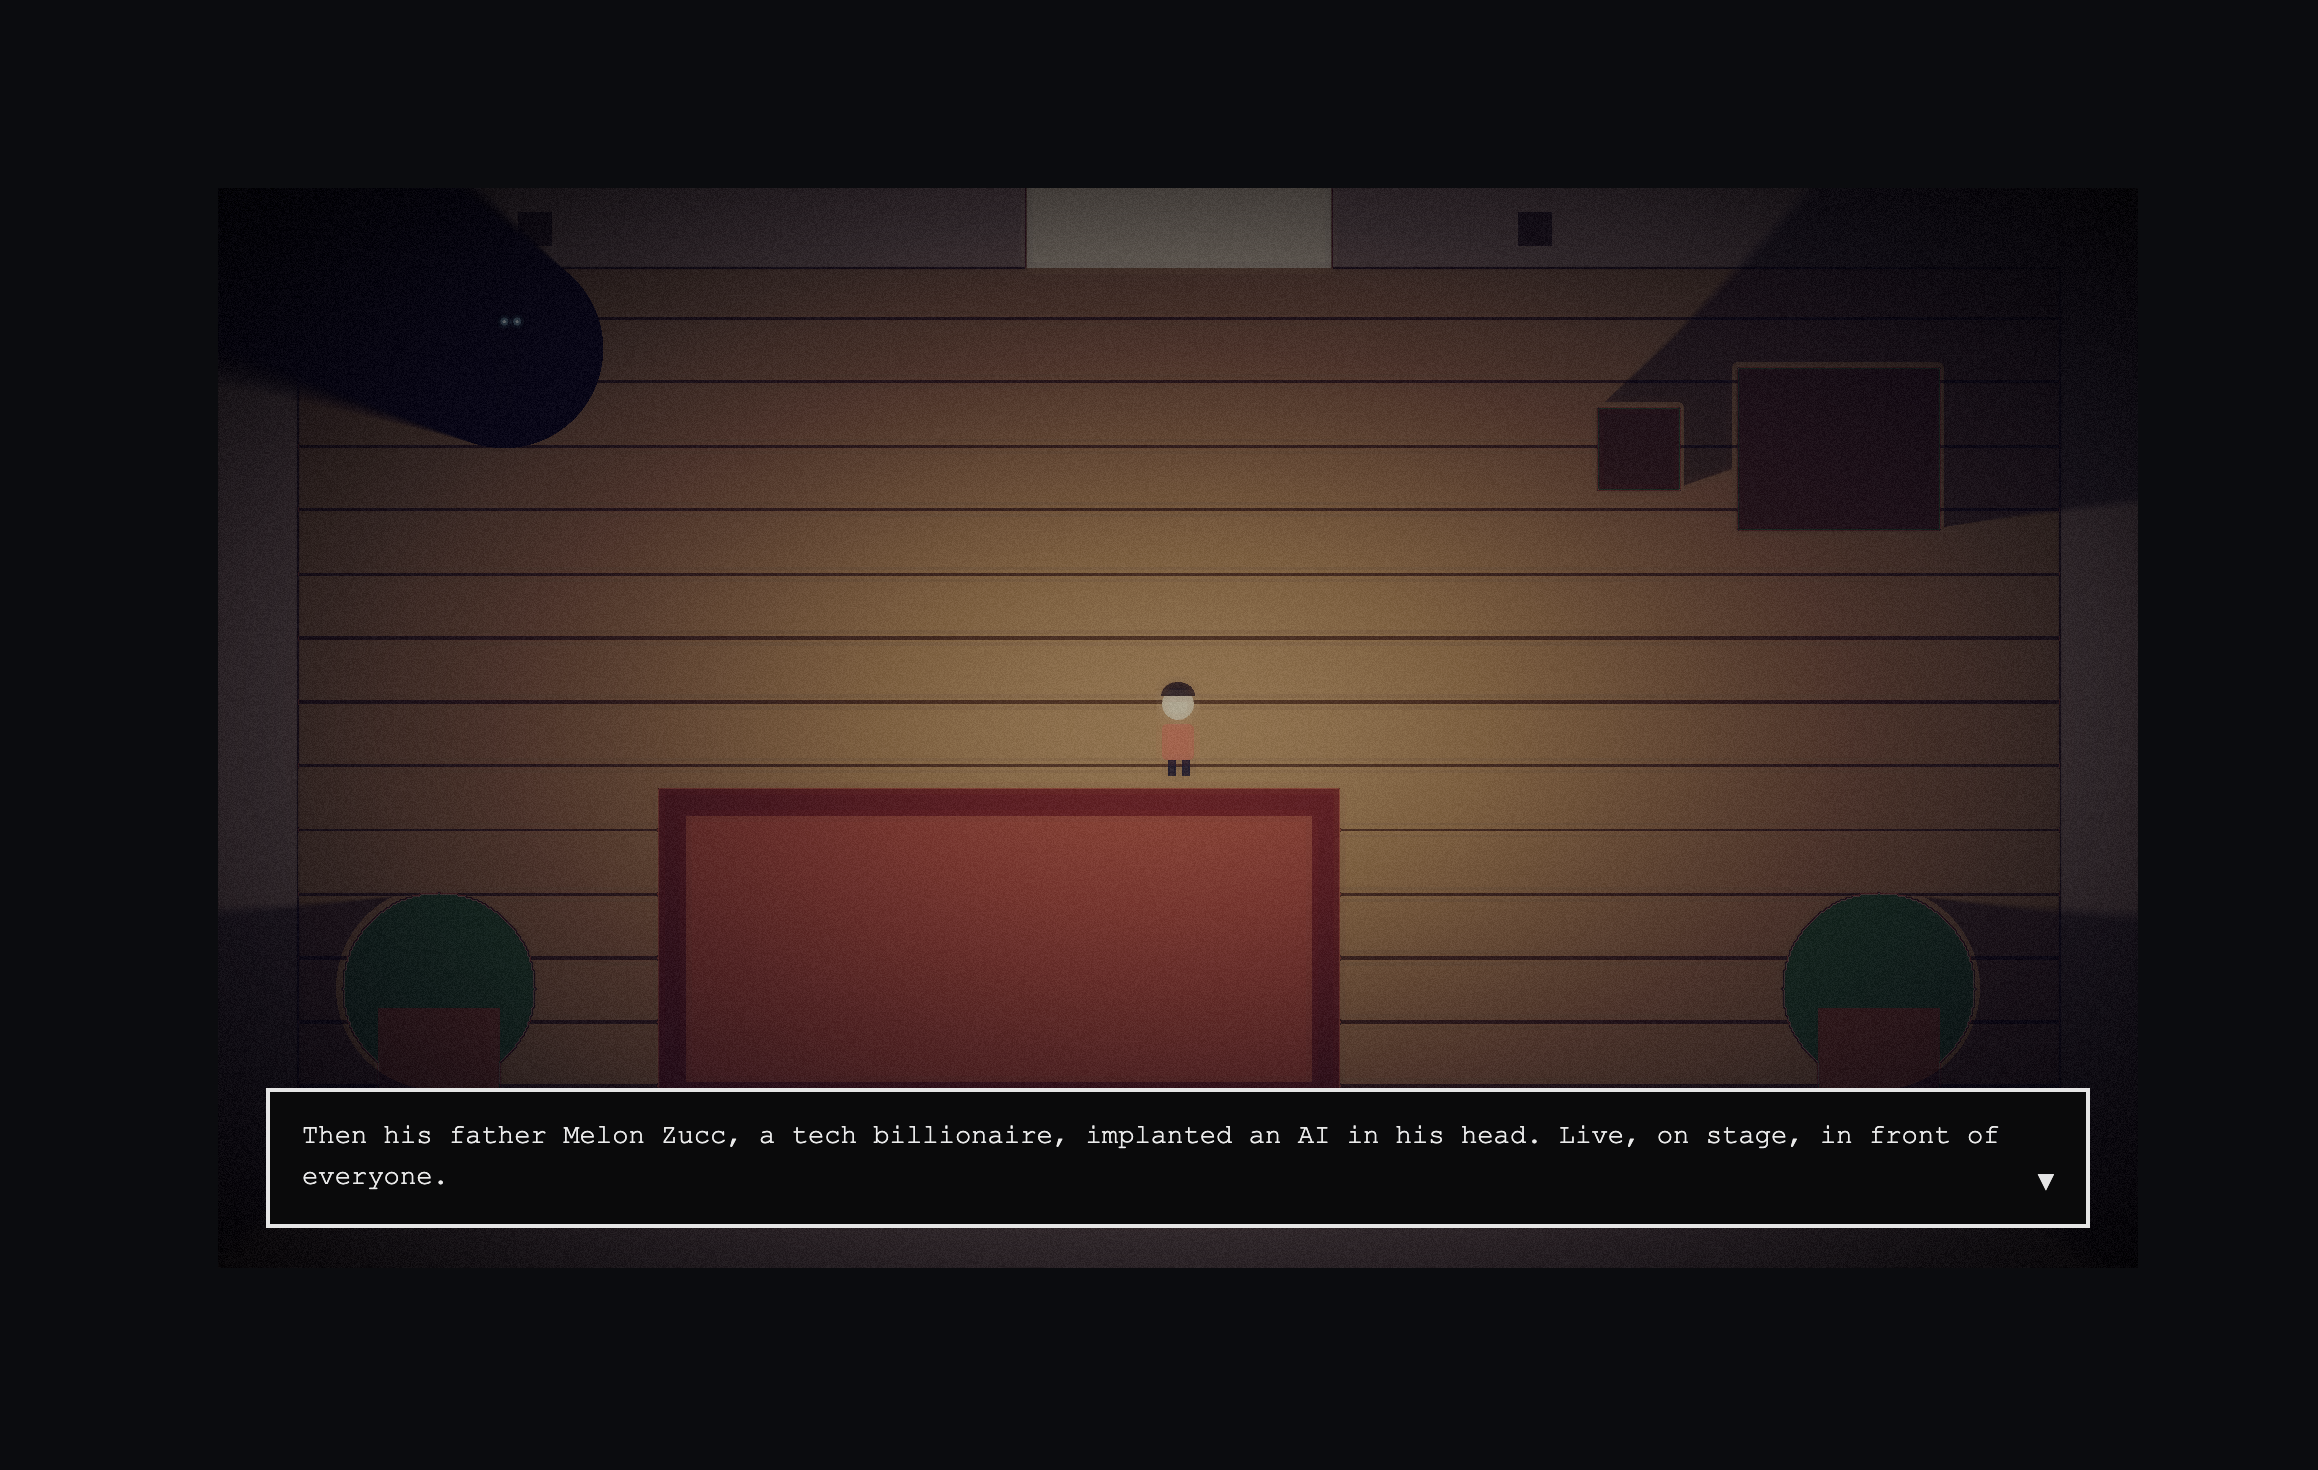
\includegraphics[width=\linewidth]{figures/hero-screenshot.png}
  \caption{The intro sequence in the running build: the player sprite in the lit environment, showing Sobel-derived N$\cdot$L shading across the distinct wood-plank, plant, and photo-frame materials read from the height map's colour bands. The antagonist's glowing-eyed silhouette is visible at top left, already present before the chase begins.}
  \label{fig:hero}
\end{figure}

\section{Background and Related Work}
This project sits at the intersection of four areas:

\begin{itemize}
  \item \textbf{Real-time rendering techniques} (lighting/shading, shadows, tone mapping) commonly used in interactive graphics \cite{akenine2018realtime,quilez2010softshadows,hart1996spheretracing,reinhard2002tonereproduction}.
  \item \textbf{Signed distance field rendering / sphere tracing} as a compact procedural geometry and rendering approach \cite{hart1996spheretracing,quilez2010softshadows}.
  \item \textbf{Human--computer interaction and the cultural framing of conversational systems}, specifically how people attribute intelligence or agency, and how social context shapes interpretation \cite{turing1950computing,turkle2011alone}.
  \item \textbf{Perceptual and visual communication foundations} relevant to composition and how viewers read images \cite{arnheim1954art}.
\end{itemize}

One additional source on procedural game-feel design was consulted early in the project but excluded from this bibliography after its bibliographic record could not be independently verified as a stable, citable publication; its content is not relied on anywhere in this report.

\section{Technical Contribution}
This section distinguishes the project from assembling equivalent functionality in Unity or Unreal via built-in renderers and post-processing stacks.

\subsection{Contributions}
\begin{itemize}
  \item \textbf{A custom real-time rendering pipeline}: explicit implementation and tuning of shading, shadowing, and tone-mapping steps rather than relying on engine defaults, with design-motivated parameters and constraints \cite{akenine2018realtime,reinhard2002tonereproduction}.
  \item \textbf{A procedural SDF raymarching approach}: sphere tracing used for both the dynamic antagonist and static scene geometry, producing soft-shadow approximations within a single shared shadow pass \cite{hart1996spheretracing,quilez2010softshadows}.
  \item \textbf{Design-driven visual perception framing}: purposeful control of contrast, luminance mapping, and composition to support readability and mood \cite{reinhard2002tonereproduction,arnheim1954art}.
\end{itemize}

\subsection{Non-goals}
The project is not a general-purpose engine or editor, and does not attempt photorealistic global illumination; effects are chosen for clarity, performance, and authorial control over physical accuracy.

\subsection{Implementation-status policy}
Any technique described in this report as ``implemented'' is confirmed working in the running build at time of writing. Techniques that were attempted and abandoned, or that remain partially working, are labeled as such explicitly (see Section~\ref{sec:discussion}).

\section{Rendering Techniques}
This section covers only techniques actually present in the build, each with a primary-source citation.

\subsection{Shading: diffuse and procedural normals}
Lambertian diffuse ($N\cdot L$) is the baseline diffuse model used throughout \cite{akenine2018realtime}. Rather than authoring a normal map texture, the environment provides a greyscale height map; a Sobel kernel evaluated per-fragment converts local height gradients directly into a surface normal, a classical image-gradient technique rather than a tangent-space normal-mapping method, since no mesh or precomputed tangent basis exists anywhere in this pipeline:

\begin{lstlisting}[language=GLSL,caption={Sobel-derived normal, then Lambertian diffuse against a moving point light.},label={lst:sobel}]
float Gx = (-tl - 2.0*l - bl + tr + 2.0*r + br) * 0.1;
float Gy = ( tl + 2.0*t + tr  - bl - 2.0*b - br) * 0.1;
vec3 normal = normalize(vec3(-Gx, -Gy, 1.0));

vec3 lightDir = normalize(vec3(uMouse, 0.5) - vec3(vTexCoord, 0.0));
float NdotL = max(dot(normal, lightDir), 0.0);
\end{lstlisting}

The same height-map texture is read a second time for its raw value (not its gradient) to select a per-material albedo colour, so one texture drives both the surface normal and the surface's base colour.

\subsection{Shadows: two raymarched SDFs, not one}
The antagonist and static furniture use the same Quilez soft-shadow near-miss estimator \cite{quilez2010softshadows}, itself built on the sphere-tracing principle of stepping by the SDF value rather than a fixed increment \cite{hart1996spheretracing}. An earlier plan to merge both into a single scene distance field (one \texttt{min()}-combined SDF, raymarched once) was abandoned in favor of raymarching each separately, once per fragment:

\begin{lstlisting}[language=GLSL,caption={Two independent raymarches, combined by taking the minimum of the resulting shadow factors, not by merging the distance fields themselves.},label={lst:raymarch}]
float shadowCharlie = raymarch(p0, lightPx, false);

float shadowFurniture = 1.0;
if (furnitureSDF(p0) > 3.0) {          // skip the self-shadow zone
  shadowFurniture = raymarch(p0, lightPx, true);
  shadowFurniture = max(shadowFurniture, 0.6);
}
float shadow = min(shadowCharlie, shadowFurniture);
\end{lstlisting}

The split exists because furniture needed two things the antagonist doesn't: an exclusion test near its own surface to avoid self-shadowing (Section~\ref{sec:discussion}), and a lighter darkness floor so its shadows read as present without going full black. Combining shadow \emph{factors} with \texttt{min()} after two raymarches, rather than combining \emph{distances} before one, is a real divergence from the single-scene-SDF design described elsewhere in this report and worth stating plainly rather than leaving the simpler-sounding version uncorrected.

\subsection{Tone mapping and post-processing}
The composited scene passes through a single post shader applying, in order: a 9-tap bloom threshold extraction, Reinhard photographic tone mapping \cite{reinhard2002tonereproduction} to compress the boosted-exposure result back into displayable range, a shadow-tint colour grade, a smoothstep vignette, and hash-based film grain. Ordering matters: grain is applied after tone mapping so it is not itself compressed in the highlights.

\subsection{Supplementary: procedural audio}
Not a primary contribution: the technical core remains the rendering pipeline above. Atmosphere is reinforced by a spatial drone synthesized from raw Web Audio API oscillator, gain, and stereo-panner nodes (no samples), panned toward the antagonist and intensifying with proximity, connecting to the horror-through-implication design discussed in Section~\ref{sec:ethics}; Grimshaw's audio uncanny valley concept (sound that implies a threat without confirming it) is the closest fit \cite{grimshaw2009audiouncanny}.

\section{System Overview}
The application is a static site (p5.js, WEBGL mode, no build step), split into a GitHub Pages blog and the game itself. This section describes the game's implemented architecture.

\subsection{Render loop}
Each frame runs three shader passes into one off-screen framebuffer, since no single shader pass can compute lighting, shadowing, and post-processing simultaneously: each stage requires the previous stage's completed output as an input texture:

\begin{figure}[t]
\centering
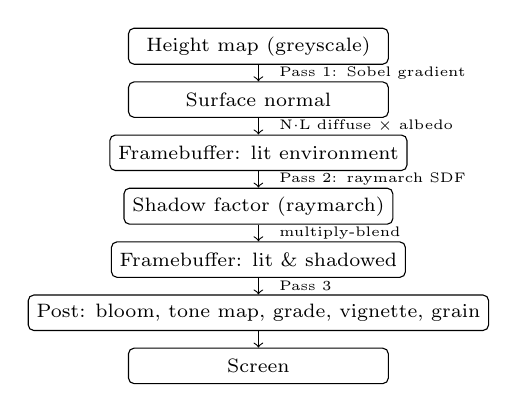
\begin{tikzpicture}[
  node distance=6pt,
  box/.style={draw, rounded corners=2pt, minimum width=3.3cm, minimum height=0.45cm, align=center, font=\scriptsize, inner sep=3pt},
  lbl/.style={font=\tiny, align=left, text width=2.6cm}
]
\node[box] (hm) {Height map (greyscale)};
\node[box, below=of hm] (norm) {Surface normal};
\node[box, below=of norm] (fb1) {Framebuffer: lit environment};
\node[box, below=of fb1] (shadow) {Shadow factor (raymarch)};
\node[box, below=of shadow] (fb2) {Framebuffer: lit \& shadowed};
\node[box, below=of fb2] (post) {Post: bloom, tone map, grade, vignette, grain};
\node[box, below=of post] (screen) {Screen};

\draw[->] (hm) -- (norm) node[lbl, midway, right=4pt] {Pass 1: Sobel gradient};
\draw[->] (norm) -- (fb1) node[lbl, midway, right=4pt] {N$\cdot$L diffuse $\times$ albedo};
\draw[->] (fb1) -- (shadow) node[lbl, midway, right=4pt] {Pass 2: raymarch SDF};
\draw[->] (shadow) -- (fb2) node[lbl, midway, right=4pt] {multiply-blend};
\draw[->] (fb2) -- (post) node[lbl, midway, right=4pt] {Pass 3};
\draw[->] (post) -- (screen);
\end{tikzpicture}
\caption{The three-pass render loop. Each box is a framebuffer state; each arrow is the shader stage that produces it from the state above.}
\label{fig:pipeline}
\end{figure}

\subsection{Interaction loop}
\label{sec:interaction}
A small state machine (\texttt{start} $\to$ \texttt{intro} $\to$ \texttt{playing} $\to$ \texttt{confront} $\to$ \texttt{choice} $\to$ \texttt{ending}) gates gameplay logic. During \texttt{playing}, keyboard input updates the player's position, which drives both the light source in Pass~1 and the pursuit target for the antagonist's steering behaviour:

\begin{lstlisting}[language=GLSL,caption={A three-stage speed model: a slow opening, a ramp toward a target duration, and a late rubber-band spike if the player is pulling away as time runs low.},label={lst:pursuit}]
const rampT = constrain(
  (elapsedSeconds - CHARLIE_SLOW_PHASE_SECONDS) /
  (CHASE_TARGET_SECONDS - CHARLIE_SLOW_PHASE_SECONDS), 0, 1);
let charlieSpeed = lerp(CHARLIE_SPEED_BASE, CHARLIE_SPEED_MAX, rampT);

if (elapsedSeconds >= closingWindowStart) {
  if (rubberbandDistRef === null) rubberbandDistRef = dist;
  if (dist > rubberbandDistRef) charlieSpeed *= RUBBERBAND_BOOST;
}
\end{lstlisting}

`charlieSpeed` is built from three stages, tuned after playtesting made a first version (a flat 25-second ramp) feel wrong: for the first \texttt{CHARLIE\_SLOW\_PHASE\_SECONDS} (10s), Charlie holds near his base speed, giving the player room to explore before any real pressure starts. From there, speed ramps linearly toward a value slightly above player speed by around \texttt{CHASE\_TARGET\_SECONDS} (25s), aiming for a full chase in the 20 to 30 second range. In the final \texttt{RUBBERBAND\_WINDOW\_SECONDS} (8s) before that target, a rubber-band check snapshots the player's distance from Charlie at the moment that window opens; if the player has since pulled further away, evading well right as time is running out, Charlie's speed gets a \texttt{RUBBERBAND\_BOOST} (1.6$\times$) spike on top of the ramp, which is what stops a well-evading player from simply outrunning him forever. Distance between player and antagonist also drives the shadow raymarcher's radius uniform and a capped ``fake-out'' event, in which the antagonist's position uniform is temporarily pushed off-canvas so it briefly disappears from both the sprite layer and the shared shadow SDF before reappearing elsewhere in the room.

\subsection{Dialogue}
A typewriter-effect dialogue engine drives the intro exposition, confrontation, and ending, rendered as a DOM overlay above the canvas rather than in-canvas WEBGL text, after an early attempt at the latter disturbed shader pipeline state. Per the original narrative design, both branches of the confrontation's binary choice converge to the same ending, since the branch itself is not part of the graded technical contribution.

\section{Evaluation Plan}
\label{sec:evaluation}
Full consent text and rating sheet are maintained separately (\texttt{user-study-form.md}) and summarised here; raw per-participant response data is in \texttt{user-study-data/}. The study is a within-subjects comparison ($n \geq 5$, counterbalanced order) between the full lit pipeline and a flat/unlit control condition reached via a URL parameter that strips only the N$\cdot$L and shadow terms; room layout, characters, audio, and post-processing are identical in both conditions, isolating the rendering technique itself as the variable under test. The Self-Assessment Manikin (valence, arousal, dominance) \cite{bradleylang1994sam} is administered after each condition, alongside two short open questions.

\begin{figure*}[t]
  \centering
  \begin{minipage}{0.48\linewidth}
    \centering
    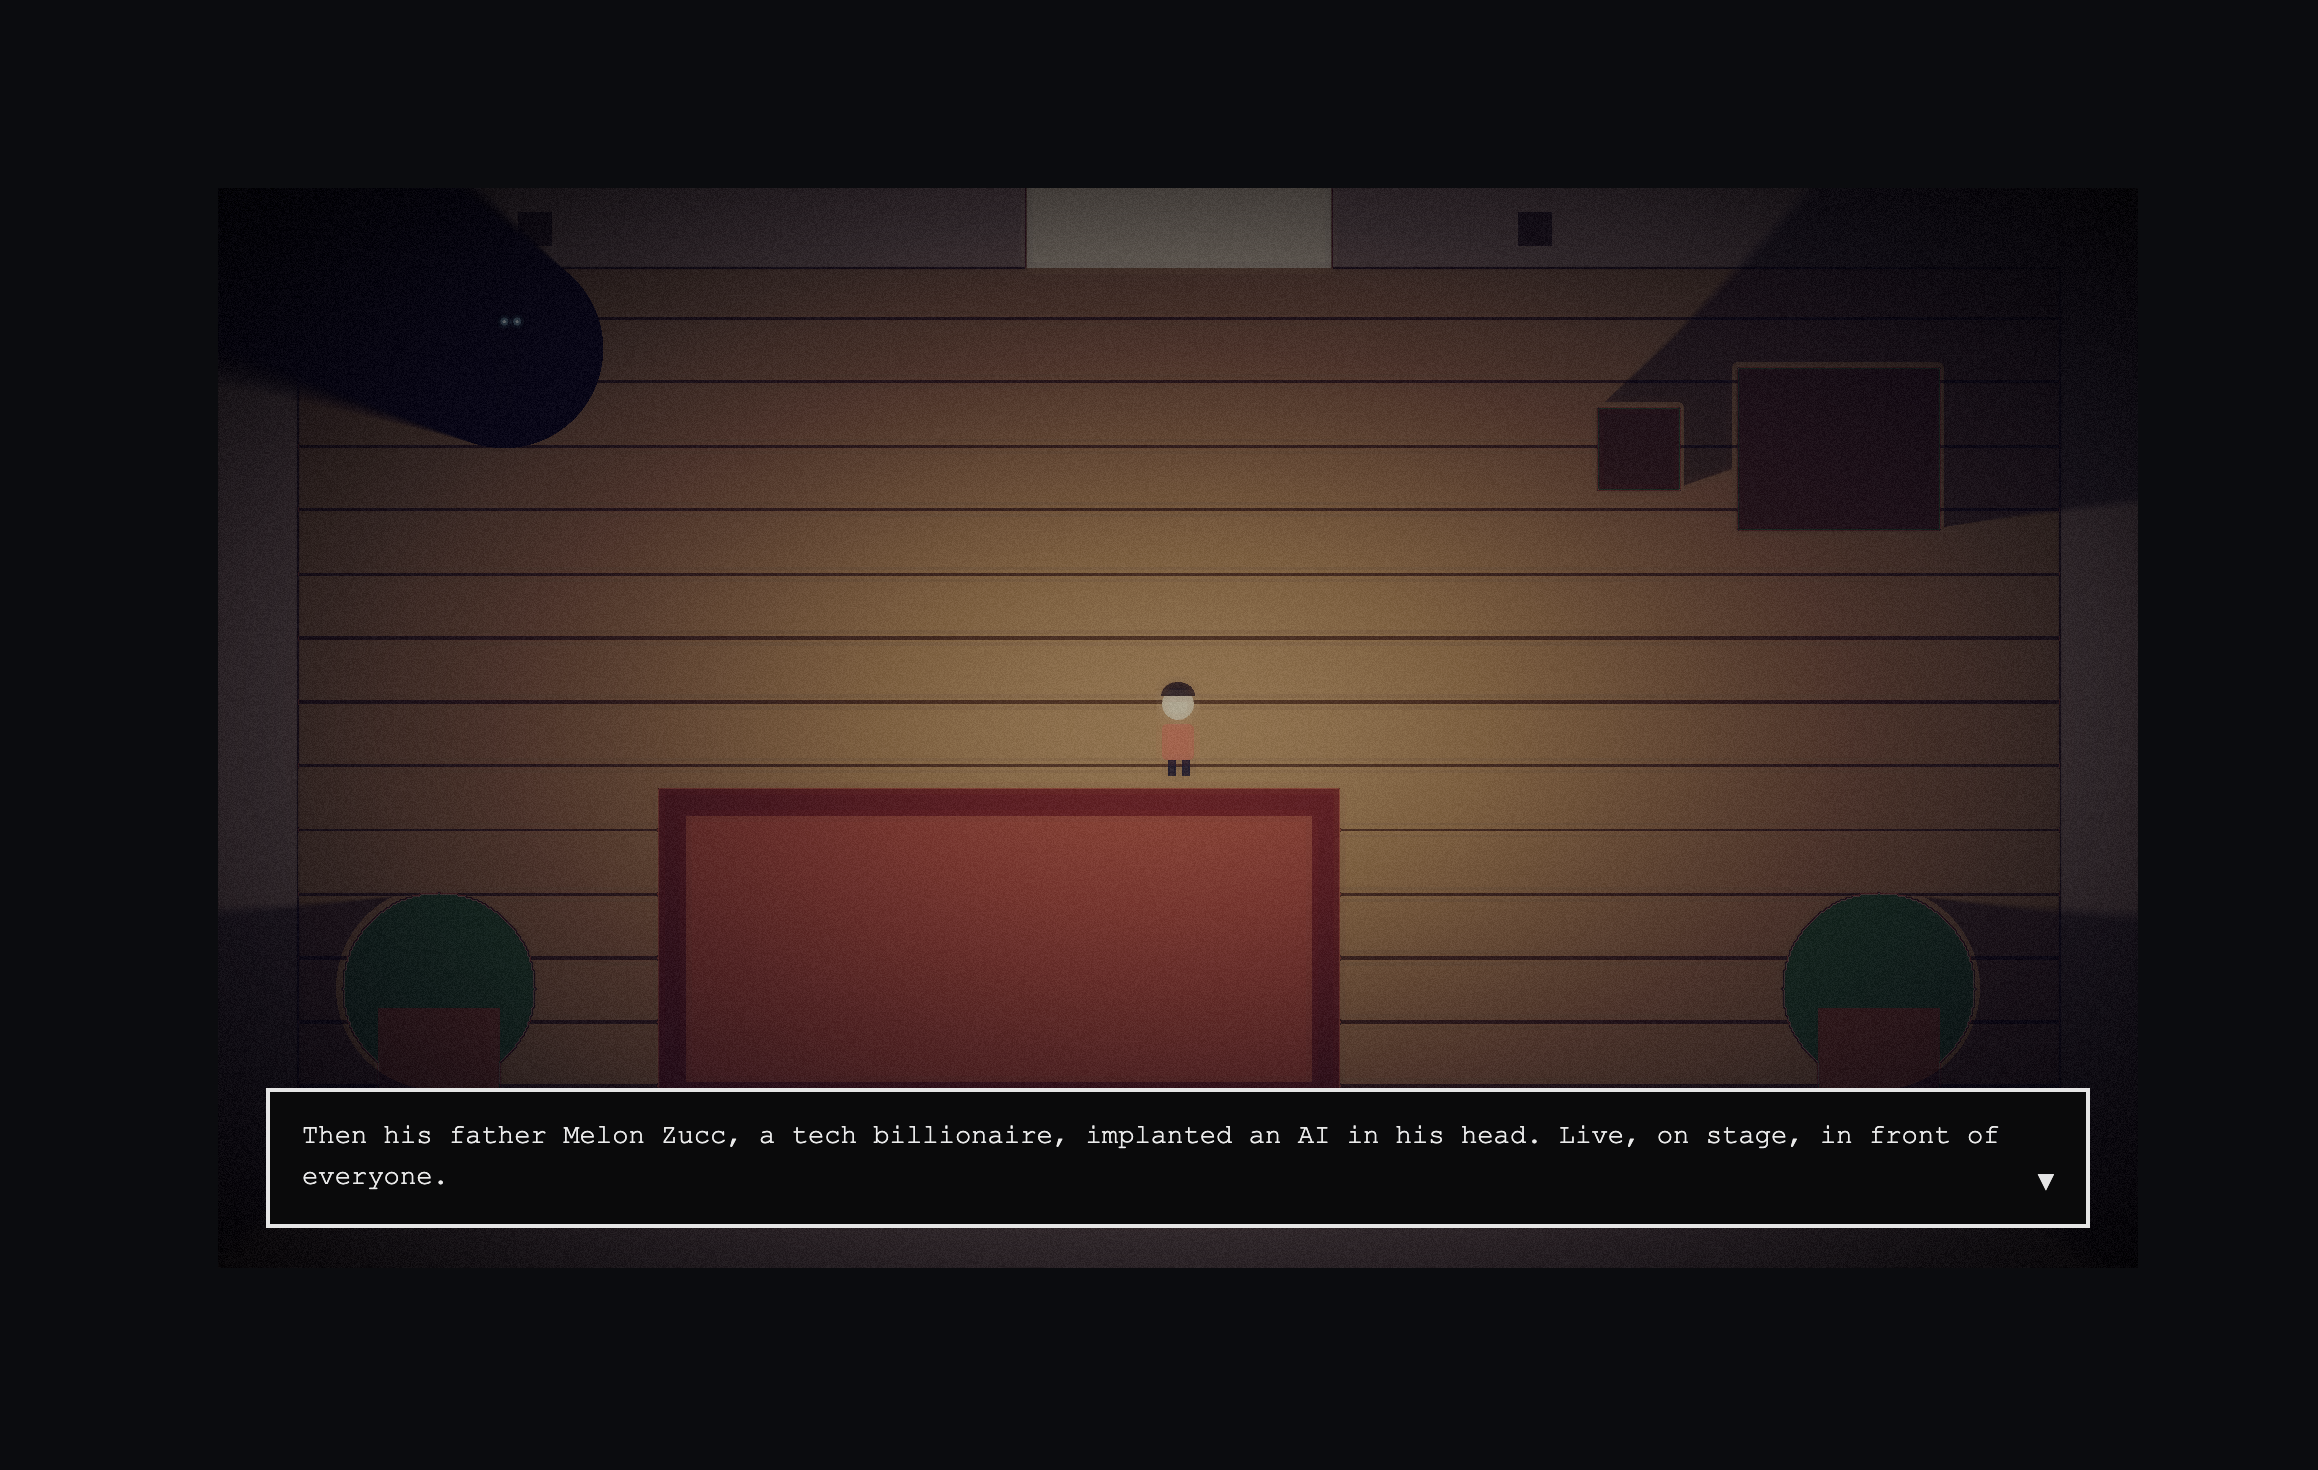
\includegraphics[width=\linewidth]{figures/hero-screenshot.png}\\[2pt]
    {\footnotesize Lit condition}
  \end{minipage}\hfill
  \begin{minipage}{0.48\linewidth}
    \centering
    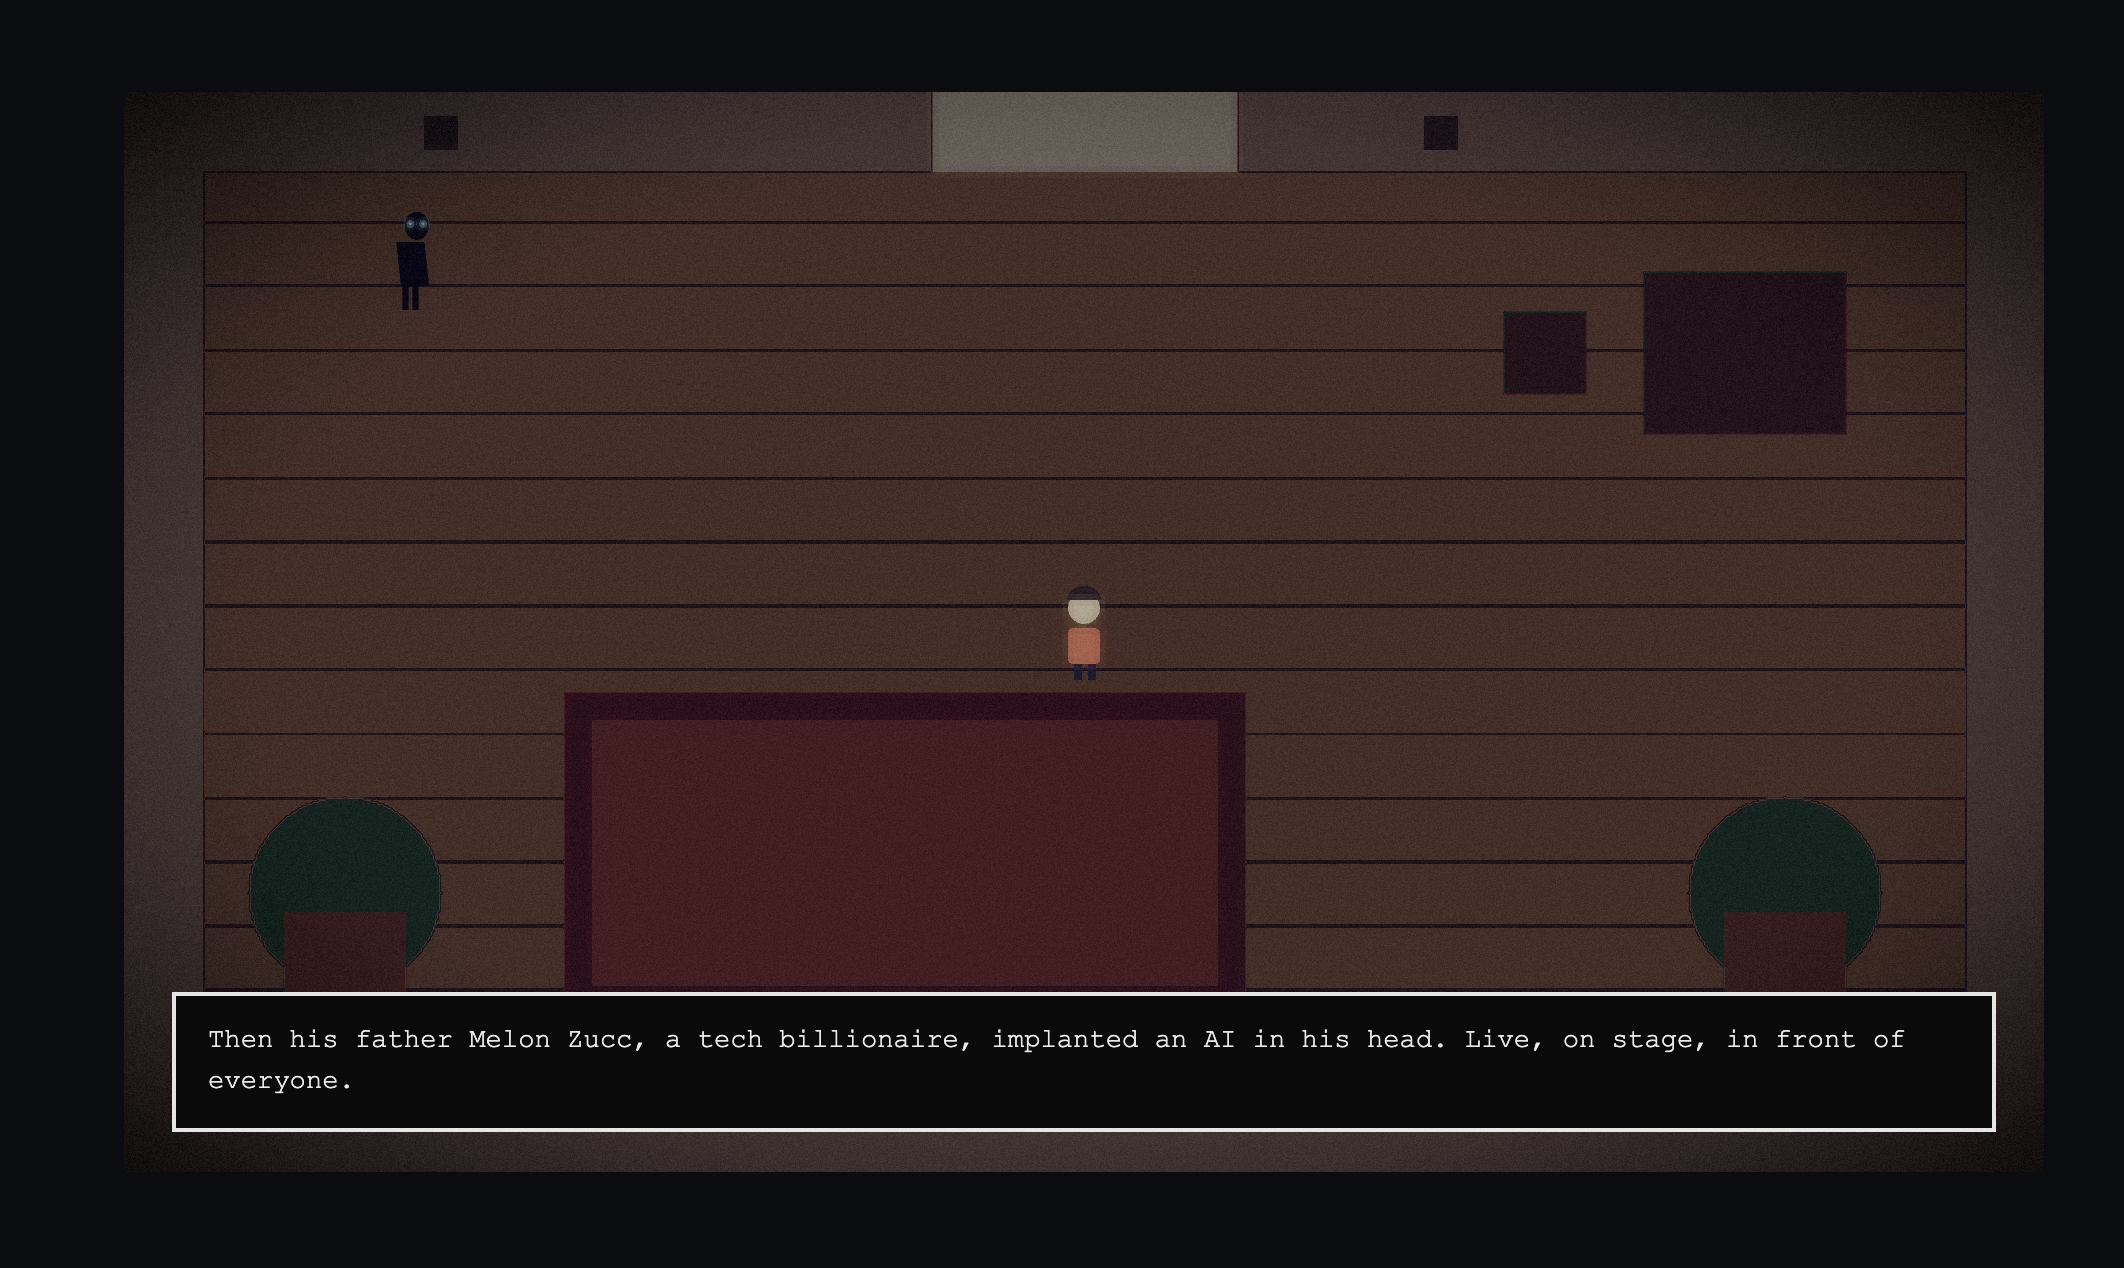
\includegraphics[width=\linewidth]{figures/flat-mode.png}\\[2pt]
    {\footnotesize Flat condition (\texttt{?mode=flat})}
  \end{minipage}
  \caption{The same moment under both study conditions. Only the N$\cdot$L diffuse and shadow terms differ; room layout, the antagonist's position, materials, and post-processing are identical, isolating the rendering technique as the variable under test.}
  \label{fig:flatvslit}
\end{figure*}

\subsection{Results ($n = 8$)}
Full per-participant data: \texttt{user-study-data/} (raw Google Form CSV exports). $n = 8$ (5 lit-first, 3 flat-first), collected through the study's Google Form.

\begin{center}
\begin{tabular}{@{}lccc@{}}
\toprule
Dimension & Lit (M $\pm$ SD) & Flat (M $\pm$ SD) & Diff (L $-$ F) \\
\midrule
Valence   & 5.63 $\pm$ 2.33 & 4.50 $\pm$ 2.07 & $+1.13$ \\
Arousal   & 6.13 $\pm$ 2.70 & 5.00 $\pm$ 3.07 & $+1.13$ \\
Dominance & 4.38 $\pm$ 2.13 & 4.25 $\pm$ 2.49 & $+0.13$ \\
\bottomrule
\end{tabular}
\end{center}

The directional pattern is the same across all three dimensions: the lit condition scored higher, not lower, than flat, the opposite of the naive prediction that better lighting should read as more unpleasant or more threatening. What it more likely reflects is that the flat condition felt less like a coherent scene and more like an abstract, disorienting one, which participants described as unsettling in a different way rather than simply less scary. A Wilcoxon signed-rank test on Valence, the only dimension with no tied or zero paired differences at this $n$, gives $W = 10.5$ ($n=8$), not significant at $\alpha = .05$. Arousal and Dominance both had 4 of 8 participants report exactly zero difference between conditions, a real finding in its own right, but too few non-zero pairs remain for a meaningful test on those two; they are reported descriptively only. Consistent with the protocol's own framing, this is exploratory: a directional signal worth reporting, not a powered significance result.

Representative quotes:
\begin{itemize}
  \item ``The unlit version felt more scary because it seemed more cold and unrealistic. Second one also felt less scary because I already knew the scene.'' This participant played flat first, then lit, and names a genuine confound the design tries to control for but cannot fully remove: familiarity with the room's layout on a second playthrough plausibly reduces tension regardless of which condition comes second.
  \item ``More creepy with no light, you see everything flat, creepier when I see it walking around compared to heavy darkness like a blob.'' A different participant's read on the same trade-off: the lit condition's shadow rendering obscures the antagonist into an ambiguous mass, while flat rendering shows him plainly, and for this participant the plain version was the more unsettling one, a genuine counterpoint to the pipeline's own design thesis.
  \item ``The sound had more of an impact in the second version. When most of the screen is obscured, my mind feels quieter, I abstract on the rest and focus on the danger. The dynamic lighting was also impactful, as it wasn't a predictable, constant switch on-off of the lights. It varied, with the evolving speed, making it weirder, more mysterious.'' This one supports the design thesis directly: the shadow radius tied to the antagonist's approach speed (Section~\ref{sec:interaction}) reads to this participant as unpredictable in a way a fixed on/off light would not.
\end{itemize}

Taken together, the quotes matter more than the numbers here: they suggest the technique changes what participants attend to (sound vs. sight, ambiguity vs. clarity) rather than uniformly amplifying fear, which the SAM means alone would not have surfaced.

\section{Discussion}
\label{sec:discussion}

\subsection{Coordinate space is not a detail}
The clearest failure mode encountered was computing SDF distances directly in normalized UV space (0--1 on both axes) against a non-square $960\times540$ canvas. Since a unit of UV-$x$ and a unit of UV-$y$ map to different pixel counts, distances computed this way are implicitly stretched along whichever axis is shorter in real pixels. This went unnoticed for a circular SDF but was immediately visible once rectangular furniture SDFs were added, rendering as stretched diagonal wedges rather than the shapes of the objects casting them. The fix (converting all distance math to pixel space by multiplying UV coordinates by the resolution uniform before use) is simple once identified, but illustrates that SDF techniques assume an isotropic metric space, which a screen-space canvas only provides if it happens to be square.

\subsection{Self-shadowing is structural, not an edge case}
Any pixel lying on or inside an occluder's own surface is, by the definition of a signed distance field, at or near zero distance from that occluder. A raymarch starting at such a pixel immediately reads as blocked. This was invisible for the antagonist, whose 2D silhouette sprite is drawn on top of the shadow pass and physically occludes the artifact, but fully visible for furniture, which has no equivalent covering sprite. This suggests a general rule for combining raymarched shadows with rasterized geometry: either every occluder needs a covering sprite or mesh, or the raymarch needs an explicit exclusion test near the caster's own surface: the two techniques are not naturally compatible without one of these accommodations.

\subsection{Procedural sprites vs. authored art}
Every character and furniture piece is drawn with primitive shapes rather than image assets, keeping the ``no black-box assets'' constraint consistent across the entire pipeline. This is a real trade-off against visual fidelity: authored sprites communicate character identity at a glance, while the procedural approach depends on silhouette, motion, and glow cues to convey the same information. Given course feedback that character/story design is not part of the graded contribution, this trade-off favors traceability to code over asset polish.

\subsection{Chase pacing as a design parameter, not just a bug fix}
The initial fixed speed differential (player at 0.003, antagonist at 0.0008, roughly 4$\times$ slower) made the chase literally unwinnable by evasion, so the only way to reach an ending was to walk toward the antagonist on purpose. A flat 25-second ramp fixed that, but felt wrong once playtested in the other direction: no distinction between ``just started'' and ``about to be caught,'' and no room for the environment to actually be noticed before the pressure began. The current three-stage model, detailed in Section~\ref{sec:interaction} (Listing~\ref{lst:pursuit}), separates ``give the player room to look around'' from ``make sure a good player cannot simply outrun the mechanic forever'' instead of collapsing both into one linear curve. Getting the pacing right, not merely resolvable, is what makes the ``the math does the horror automatically'' design thesis true at the level of an entire playthrough, not just a single frame's shadow radius.

\subsection{Limitations}
\begin{itemize}
  \item A single dynamic point light is sufficient for this project's mechanic but does not generalize to multi-light scenes without restructuring the diffuse pass.
  \item The evaluation (Section~\ref{sec:evaluation}) is explicitly exploratory at $n=8$; findings are suggestive, not statistically conclusive.
  \item Equipment consistency held only partially: all 8 sessions were moderated (the researcher present throughout), but some were in-person on shared equipment and others were synchronous online with the participant screen-sharing from their own device, screen, and speakers.
  \item Bloom is a single-pass 9-tap approximation, not a multi-radius Gaussian bloom.
  \item Shadow softness is currently a fixed constant per occluder type (sharp for the antagonist, floored/soft for furniture) rather than a continuous material property.
\end{itemize}

\subsection{Citation corrections (2026-08-27)}
A pass comparing this report and the project's blog diary against the running code found three references that didn't hold up, since removed from \texttt{references.bib}: Holopainen's \emph{Foundations of Gameplay}, never verified as a citable publication and never actually cited in-text; Fernando's \emph{GPU Gems}, cited only for shadow mapping / percentage-closer filtering, a technique this project does not implement (the only shadow method is the Quilez SDF raymarch above); and Schüler's tangent-space normal-mapping paper, cited for the Sobel-derived normals even though that paper solves a different problem (a TBN basis for 3D meshes) than the screen-space height-map gradient actually used here. The techniques genuinely implemented remain correctly cited; the citations that didn't match what the code does were removed rather than kept for the sake of a longer bibliography.

\section{Ethical and Societal Reflection}
\label{sec:ethics}
Conversational AI systems can be misread by users as having genuine understanding or intent; framing and disclosure matter in how such systems are presented \cite{turing1950computing,turkle2011alone}. The project's central mechanic (an antagonist that is simultaneously an AI assistant and a rendering artifact with no fixed visual form) deliberately engages this ambiguity rather than resolving it. Separately, visual design decisions (colour grade, contrast, vignette) are not neutral: they actively shape a viewer's interpretation and emotional response to a scene \cite{arnheim1954art}, which is the premise the evaluation in Section~\ref{sec:evaluation} attempts to test directly rather than assume.

\section{Conclusion}
The project demonstrates a complete procedural rendering pipeline (Sobel-derived normals, N$\cdot$L diffuse, a shared SDF soft-shadow raymarcher covering both dynamic and static geometry, and multi-effect post-processing) built entirely from first principles rather than engine defaults or pre-authored assets. Two structural bugs encountered along the way (coordinate-space anisotropy, SDF self-shadowing) are documented as general lessons rather than incidental fixes. The evaluation study (Section~\ref{sec:evaluation}), designed to isolate the rendering technique itself rather than the experience as a whole, ran at $n=8$: a directional signal across all three SAM dimensions favoring the lit condition, not statistically powered at this sample size, alongside qualitative responses suggesting the technique changes what players attend to rather than uniformly amplifying fear.

\bibliographystyle{IEEEtran}
\bibliography{references}

\end{document}
